%\documentclass[a4paper,twoside]{article}
\documentclass[14pt]{extarticle}
\usepackage[letterspace=-1000]{microtype}
\usepackage{enumerate}
\usepackage{verse}
\usepackage{ccaption}
\usepackage{fancyvrb}
\usepackage[margin=2cm]{geometry}

\usepackage{csquotes}
\usepackage[utf8x]{inputenc}
%\usepackage[cp1251]{inputenc}
\usepackage[T2A]{fontenc}
\usepackage{array}
\usepackage{amssymb}
\usepackage{amsmath}
\usepackage{amsthm}
\usepackage{latexsym}
\usepackage{indentfirst}
\usepackage{bm}
\usepackage{enumerate}
\usepackage{graphicx}
\usepackage{epsf}
%\usepackage{epsfig}
%\DeclareGraphicsExtensions{.pdf,.png,.jpg}
\usepackage{wrapfig}
\usepackage{euscript}
\usepackage{indentfirst}
\usepackage[english,russian]{babel}
\usepackage{microtype}

\newcommand{\M}{{\mathsf M}\,}
\newcommand{\cov}{\mathsf{cov}}
\newcommand{\corr}{\mathsf{corr}}
\newcommand{\var}{\mathsf{D}\,}
\renewcommand{\Pr}{{\mathsf P}}
% \sloppy\unitlength=.24mm
% \renewcommand{\thefootnote}{\arabic{footnote}}

% \textwidth=132mm
% \headheight=7mm
% \headsep=5mm
% \textheight=200mm
% \oddsidemargin=0mm
% \evensidemargin=0mm
% \topmargin=0mm

\newcommand{\firstheader}[1]{\noindent\textbf{#1}\nopagebreak\bigskip}
\newcommand{\header}[1]{\bigskip\medskip\noindent\textbf{#1}\nopagebreak\bigskip}
\newcommand{\subheader}[1]{\bigskip\medskip\noindent\emph{#1}\nopagebreak\bigskip}
\newcommand{\subsub}[1]{\bigskip\medskip\noindent\emph{#1}\nopagebreak\bigskip}
\newcommand\setItemnumber[1]{\setcounter{enumi}{\numexpr#1-1\relax}}

\newcommand{\actualityTXT}{Актуальность темы исследования.}
% степень ее разработанности;
\newcommand{\progressTXT}{Степень разработанности темы.}
% цели и задачи;
\newcommand{\aimTXT}{Цели и задачи работы.}
\newcommand{\tasksTXT}{задачи}
% научную новизну;
\newcommand{\noveltyTXT}{Научная новизна.}
% теоретическую и практическую значимость работы;
%\newcommand{\influenceTXT}{Теоретическая и практическая значимость}
% или чаще используют просто
\newcommand{\influenceTXT}{Теоретическая и практическая значимость.}
% методологию и методы исследования;
\newcommand{\methodsTXT}{Mетодология и методы исследования.}
% положения, выносимые на защиту;
\newcommand{\defpositionsTXT}{Основные положения, выносимые на~защиту.}
% степень достоверности и апробацию результатов.
\newcommand{\reliabilityTXT}{Достоверность}
\newcommand{\probationTXT}{Степень достоверности и апробация результатов.}

\newcommand{\contributionTXT}{Личный вклад автора.}
\newcommand{\publicationsTXT}{Публикации.}


\newcommand{\authorbibtitle}{Публикации автора по теме диссертации}
\newcommand{\fullbibtitle}{Список литературы} % (ГОСТ Р 7.0.11-2011, 4)



\theoremstyle{theorem}
\newtheorem{theorem}{Теорема}
\newtheorem{Theorem}{Теорема}
\newtheorem{definition}{Определение}
\newtheorem{Def}{Определение}
\newtheorem{corollary}{Следствие}
\newtheorem{proposition}{Предложение}
\newtheorem{prop}{Предположение}
\newtheorem{lemma}{Лемма}
\newtheorem{assumption}{Предположение}
\newtheorem{Lemma}{Лемма}
\newtheorem{Cons}{Следствие}
\newtheorem{Proposition}{Предложение}
\newtheorem{Statement}{Утверждение}
\newtheorem{statement}{Утверждение}
\theoremstyle{remark}
\newtheorem{remark}{Замечание}
\newtheorem{Remark}{Замечание}
\newtheorem{example}{Пример}
\newtheorem{Example}{Пример}
\newtheorem{notation}{Замечание}
\newtheorem{teo}{Теорема}
\newtheorem{sled}{Следствие}
\newtheorem{sublemma}[theorem]{\indent\bf Подлемма}
\newtheorem{problem}{\indent\bf Проблема}
\newtheorem{hypothesis}{\indent\bf Гипотеза}
\newtheorem{denotation}[theorem]{\indent\bf Обозначение}
\newtheorem{thr}{Теорема}
\newtheorem{crl}[thr]{Следствие}
\newtheorem{lmm}[thr]{Лемма}
\newtheorem{qu}{Вопрос}
\newtheorem{dfn}{Определение}
\newtheorem{approval}{Утверждение}

\makeatletter
\renewcommand*{\hm}[1]{#1\nobreak\discretionary{}%
	{\hbox{$\mathsurround=0pt #1$}}{}}% перенос арифметических знаков
\newcommand{\rmnum}[1]{\romannumeral #1}
\newcommand{\Rmnum}[1]{\expandafter\@slowromancap\romannumeral #1@}
\usepackage{lipsum}
\newcommand{\Mark}{\{(\Gamma_i, \varkappa_i); \hm{} i \geqslant 0\}}
\newcommand{\MarkThree}{\{(\Gamma_i, \varkappa_{3,i}); \hm{} i \geqslant 0\}}
\renewcommand{\Pr}{{\mathbf P}}
\newcommand{\No}{\textnumero}
\usepackage[noadjust]{cite}

% нумерацию можно оставить как есть
\newcommand{\pages}{1-8}

\begin{document}

\setcounter{page}{3}
\section*{Общая характеристика работы}

%\newcommand{\actualitySynopsis}{\underline{\textbf{\actualityTXT}}}

\underline{\textbf{\actualityTXT}} Теория массового обслуживания занимается построением и анализом моделей для сложных систем, осуществляющих большое количество однотипных операций по обслуживанию различного рода требований (заявок). Первые работы в этой области были мотивированы решением прикладных задач, связанных с организацией деятельности телефонных станций в начале XX века. Задачи, поставленные и рассмотренные Ф.В.~Йоханнсеном и А.К.~Эрлангом, заложили основу для так называемой классической теории массового обслуживания (ТМО). Дальнейшее развитие этой отрасли науки связано с именами таких ученых как Ф.~Поллачек, А.Н.~Колмогоров, А.Я.~Хинчин, Б.В.~Гнеденко, И.Н.~Коваленко, К.~Пальм, Д.Дж.~Кендалл, Л.~Такач, Д.Р.~Кокс, У.Л.~Смит, Т.Л.~Саати, Л.~Клейнрок, С.Н.~Бернштейн, Н.П.~Бусленко, А.А.~Боровков, В.С.~Королюк, Г.П.~Башарин, Г.П.~Климов, Ю.В.~Прохоров, А.Д.~Соловьев,  Б.А.~Севастьянов, Н.Т.Дж.~Бейли и др. В их работах закладываются основные понятия, формируются принципы и методы решения задач ТМО. Начиная с области телефонии, результаты теории очередей находят свое применение при исследовании систем управления наземным, водным и воздушным транспортом, систем организации медицинских учреждений, биологических систем, телекоммуникационных и компьютерных систем, процессов производства сложных объектов, в финансовой сфере и т.~д.

Оптимизационные цели существуют у большинства прикладных исследований ТМО. В некоторой идеализации система массового обслуживания (СМО) есть система, которая, находясь под действием различных случайных, неопределенных, контролируемых факторов, осуществляет операции по обслуживанию требований. При этом возможно определить различные критерии эффективности осуществления операции: среднее время пребывания требования в системе, вероятность простоя обслуживающих приборов, вероятность отказа, среднее количество занятых приборов, средняя длина очереди, коэффициент загрузки системы, производительность системы и т.~д. Целью исследования таких систем является определение способов достижения наибольшей прибыли (наибольшей эффективности системы). В связи с такой постановкой задачи, ТМО неразрывно связана с отраслью исследования операций (ИО). Такая связь наблюдается, например, в работах Н.П.~Бусленко, Н.Т.Дж.~Бейли и др. Задачи ТМО в этом случае понимаются как задачи организационно-управленческого  характера, направленные на наиболее оптимальное использование ресурсов. 

Следует также обратить внимание на связь ТМО и математической кибернетики (МК). В работе А.А.~Ляпунова и С.В.~Яблонского авторы выделяют понятие управляющей системы как одно из ключевых понятий МК. Кибернетика представляется как «наука об общих закономерностях строения управляющих систем и течения процессов управления». При изучении конкретных управляющих систем кибернетика взаимодействует со многими другими областями знаний, в том числе и с ТМО. В связи с этим привлечение аппарата и результатов МК, ИО и других дисциплин представляется актуальным и позволяет получать новые результаты.

Начиная со второй половины XX века, появляются работы, посвященные теории управляемых систем обслуживания. Понятие управляемой СМО было введено О.И.~Бронштейном и В.В.~Рыковым. Отмечено, что в управляемых СМО можно выделить элементы, допускающие применение управляющих воздействий.  Каждый подобный элемент характеризуется набором параметров. Выбор значений управляющих параметров является стратегией управления. Изучению управляемых СМО  посвящены работы Н.М.~Воробьева, Б.Г.~Питтеля, А.Ф.~Терпугова, В.В.~Рыкова и др.

Тандемы систем массового обслуживания широко используются при моделировании компьютерных и коммуникационных систем, колл-центров, аварийных служб,
при планировании их мощностей, производительности и последующей оптимизации
работы. Тандем является простейшей сетью из нескольких приборов, в которой заявка после обслуживания на одном устройстве поступает в очередь на обслуживание следующим устройством. В первых работах, посвященных тандемам систем массового обслуживания, изучается распределение времени пребывания требования в системе с двумя обслуживающими устройствами. В
предположении, что промежутки времени между поступлением заявок в систему и
времени обслуживания независимы и имеют экпоненциальные законы распределения,
было показано, что время ожидания требования в очереди первого прибора стохастически не зависит от его времени ожидания в очереди второго прибора.
Основные результаты теории тандемов в случае простейших стационарных входных потоков и экспоненциального времени обслуживания получены в работах 1980-х годов. Модели с неэкспоненциальным временем обслуживания
рассмотрены в работах А.~Гомес-Коралла. Более общие модели включают в себя так называемые BMAP
(Batch Markovian Arrival Process) входные потоки, особенностью которых является
наличие корреляции количества пришедших требований в различные моменты времени. Такие потоки рассмотрены, например, в работах В.И.Клименок, А.Н.Дудина и др, где проведены аналитические рассчеты условий стационарности и изучено поведение некоторых характеристик обслуживания для некоторых частных видов входных потоков и распределений времени обслуживания для двухфазных (тандемных) систем, в том числе
с повторными попытками и нетерпеливыми требованиями. Модель последовательных перекрестков с немгновенным перемещением машин между ними была впервые
предложена в работах А.В.~Зорина. В них динамика перемещения машин
от одного перекрестка к другому задается бернулиевской случайной величиной: каждая машина с некоторой фиксированной вероятностью успевает доехать до
следующего перекрестка и с противоположной вероятностью остается «между»
ними.

Постановка задачи в первых классических работах по ТМО сводилась к поиску оптимального числа обслуживающих приборов, минимизирующего среднее время ожидания клиентов. Решение при этом находилось аналитически. Со временем системы, изучаемые методами ТМО и ИО, значительно усложнялись. В связи с этим возникает необходимость в новых критериях оценки качества функционирования системы, а также в новых методах исследования. Одним из самых распространенных методов при решении подобных оптимизационных задач на текущий момент является метод имитационного моделирования. Компьютерные имитационные модели позволяют учитывать достаточно большое число факторов, которые с трудом могут быть учтены при аналитическом исследовании в силу его возрастающей сложности. Кроме того, преимущество имитационных моделей связано с возможностью исследовать различные сценарии работы управляемых систем, сравнительно легко адаптировать модели к изменениям в физической постановке задачи. В диссертационной работе аналитические методы применяются наряду с численным исследованием путем имитационного моделирования. Такое объединение методологий представляется актуальным и увеличивает достоверность результатов.
\newcommand{\progress}{\underline{\textbf{\progressTXT}}}
\newcommand{\aim}{\underline{{\textbf\aimTXT}}}
\newcommand{\tasks}{\underline{\textbf{\tasksTXT}}}
\newcommand{\novelty}{\underline{\textbf{\noveltyTXT}}}
\newcommand{\influence}{\underline{\textbf{\influenceTXT}}}
\newcommand{\methods}{\underline{\textbf{\methodsTXT}}}
\newcommand{\defpositions}{\underline{\textbf{\defpositionsTXT}}}
\newcommand{\reliability}{\underline{\textbf{\reliabilityTXT}}}
\newcommand{\probation}{\underline{\textbf{\probationTXT}}}
\newcommand{\contribution}{\underline{\textbf{\contributionTXT}}}
\newcommand{\publications}{\underline{\textbf{\publicationsTXT}}}
%{\aim} Целями данной работы являются: 1)~построение и исследование математической модели тандема управляющих систем обслуживания по циклическому алгоритму с продлением; 2)~построение, реализация и анализ имитационной модели систем, осуществляющих циклическое управление с продлением тандемом перекрестков.

Для~достижения поставленных целей решаются следующие задачи:

1. Построение строгой вероятностной модели тандема управляющих систем с помощью явного построения вероятностного пространства и поточечного задания необходимых для исследования случайных величин и элементов.

2. Анализ построенной вероятностной модели, получение условий существования стационарного режима в различных подсистемах тандема.

3. Разработка имитационной модели тандема, определение момента достижения системы квазистационарного режима, анализ зависимости условий стационарности от управляющих параметров.



{\novelty} Основные результаты являются новыми и состоят в следующем:

1. Построена строгая вероятностная модель тандема управляющих систем с немгновенным перемещением требований между ними, управление в которых осуществляется по циклическому алгоритму и алгоритму с продлением. 

2. Изучены эргодические свойства построенной модели, найдены условия существования стационарного режима для очередей первичных требований, а также для промежуточной очереди.

3. Разработана и реализована имитационная модель для тандема

4. Проведено исследование вероятностной и имитационной моделей, и определена расширенная область стационарности системы при алгоритме с продлением.




{\influence} Научная значимость работы заключается в построении строгой вероятностной модели 
для качественно нового вида управляющей системы и в последовательном исследовании ее эргодических свойств. Успешно примененный в работе метод нелокального описания процессов существенно расширяет множество поддающихся исследованию реальных систем массового обслуживания. Строгая математическая модель позволяет оперировать существующим, хорошо разработанным вероятностным аппаратом для нахождения условий стационарности и нахождения оптимального управления системой. 
 Разработанные модели дают базу для изучения более комплексных тандемных систем, систем с более сложными входными потоками и алгоритмами управления.

Практическая значимость исследования состоит в том, что изученная управляющая система является адекватным описанием реальной системы тандема перекрестков, а также других сетей, состоящих из двух узлов с перемещающимися между ними требованиями и циклическими алгоритмами обслуживания с продлением на узлах.




{\methods} Методология диссертационной работы базируется на представлении стохастических систем массового обслуживания в виде кибернетических управляющих систем. Применение принципов кибернетического подхода позволяет выделить в изучаемых системах ключевые блоки, структурировать информацию о законах функционирования блоков и основных связях между ними. Для описания входных потоков был примен метод нелокального описания, что сделало возможным более глубокое математическое изучение рассматриваемых объектов. В работе используется аппарат теории вероятностей, теории массового обслуживания, исследования операций, теории управляемых марковских процессов, теории функций комплексного переменного. Также применяются методы математической статистики, матричных вычислений и теории систем линейных алгебраических уравнений. При разработке имитационных моделей использовался язык программирования C++. Для визуализации результатов некоторых численных исследований использовался язык Python.


{\defpositions}

1. Методика построения вероятностного пространства для тандема систем с немгновенным перемещением требований между ними.

2. Методика нахождения условий существования стационарного режима в системах управления потоками неоднородных требований с циклическим алгоритмом и алгоритмом с продлением.

3. Метод определения момента достижения управляемой системой обслуживания квазистационарного режима.





{\probation} Достоверность полученных результатов обеспечивается строгим применением используемого математического аппарата, проведением статистических и численных исследований. Результаты работы находятся в соответствии с результатами, полученными ранее другими авторами при исследовании управляющих систем обслуживания.

Основные результаты диссертации докладывались и обсуждались на следующих  конференциях.
\begin{enumerate}
    \item Международная научная конференция <<Теория вероятностей, случайные процессы, математическая статистика и приложения>> (Минск, Республика Беларусь, 2015 г.).
    \item IX Международная конференция <<Дискретные модели в теории управляющих систем>> (Москва и Подмосковье, 2015 г.).
\item 8-я международная научная конференция <<Распределенные компьютерные и коммуникационные сети: управление, вычисление, связь>> DCCN-2015 (Москва, 2015 г.).
\item Международная научная конференция <<Distributed Computer and Communication Networks>> DCCN 2016 (Москва, 2016 г.).
\item XVIII Международная конференция <<Проблемы теоретической кибернетики>> (Пенза, 2017 г.).
\item XVI Международная конференция имени А.Ф. Терпугова <<Информационные технологии и математическое моделирование>> ИТММ-2017 (Казань, 2017 г.).
\item  20-я международная научная конференция <<Распределенные компьютерные и телекоммуникационные сети: управление, вычисление, связь>> DCCN-2017 (Москва, 2017 г.).
\item IX Московская международная конференция по исследованию операций (Москва, 2018~г.).
\end{enumerate}


{\contribution} В совместных публикациях научному руководителю принадлежит постановка задачи и общее редактирование работ. Все исследования выполнены автором диссертации лично, все полученные результаты принадлежат автору. 


\ifnumequal{\value{bibliosel}}{0}{% Встроенная реализация с загрузкой файла через движок bibtex8
    \publications\ Основные результаты по теме диссертации изложены в XX печатных изданиях, 
    X из которых изданы в журналах, рекомендованных ВАК, 
    X "--- в тезисах докладов.%
}{% Реализация пакетом biblatex через движок biber
%Сделана отдельная секция, чтобы не отображались в списке цитированных материалов
    %\begin{refsection}%
        %\printbibliography[heading=countauthornotvak, env=countauthornotvak, keyword=biblioauthornotvak, section=1]%
        %\printbibliography[heading=countauthorvak, env=countauthorvak, keyword=biblioauthorvak, section=1]%
        %\printbibliography[heading=countauthorconf, env=countauthorconf, keyword=biblioauthorconf, section=1]%
        %\printbibliography[heading=countauthor, env=countauthor, keyword=biblioauthor, section=1]%
        %\publications\ Основные результаты по теме диссертации изложены в \arabic{citeauthor} печатных изданиях\nocite{bib1,bib2}, 
        %\arabic{citeauthorvak} из которых изданы в журналах, рекомендованных ВАК\cite{vestnikUNN,vestnikVGAVT1,vestnikVGAVT2,vestnikTGU}, 
        %\nocite{DCCN2010,Minsk2011,Novgorod2011,Novosibirsk2011,DCCN2013,Kazan,Minsk2015,RachinskayaStatistics,Dm2015,DCCN2015,Dm2016,Penza2017,DCCN2017,Tomsk2017,Soloviev2017}\arabic{citeauthorconf} "--- в тезисах докладов  \cite{DCCN2010,Minsk2011,Novgorod2011,Novosibirsk2011,DCCN2013,Kazan,Minsk2015,RachinskayaStatistics,Dm2015,DCCN2015,Dm2016,Penza2017,DCCN2017,Tomsk2017,Soloviev2017}.
        	\publications\ Основные результаты по теме диссертации изложены в 10 работах, 
	1 из них "--- в журнале, рекомендованном ВАК для защиты по специальности 01.01.09,
	2 "--- в библиографической базе Scopus, 2 "--- в библиографической базе Web of Science, 1 "--- в журнале, рекомендованном ВАК для защиты по смежной специальности 05.13.01, 9 "--- в библиографической базе РИНЦ,
	8 "--- в тезисах докладов. 
	%  \end{refsection}

}



 % Характеристика работы по структуре во введении и в автореферате не отличается (ГОСТ Р 7.0.11, пункты 5.3.1 и 9.2.1), потому ее загружаем из одного и того же внешнего файла, предварительно задав форму выделения некоторым параметрам


{\aim} Целями данной работы являются: 1)~построение и исследование математической модели тандема управляющих систем обслуживания по циклическому алгоритму с продлением; 2)~построение, реализация и анализ имитационной модели систем, осуществляющих циклическое управление с продлением тандемом перекрестка.

Для~достижения поставленных целей решаются следующие задачи:

1. Построение строгой вероятностной модели тандема управляющих систем с помощью явного построения вероятностного пространства и поточечного задания необходимых для исследования случайных величин и элементов.

2. Анализ построенной вероятностной модели, получение условий существования стационарного режима в различных подсистемах тандема.

3. Разработка имитационной модели тандема, определение момента достижения системы квазистационарного режима, анализ зависимости условий стационарности от управляющих параметров.


{\novelty} Основные результаты являются новыми и состоят в следующем:

1. Построена строгая вероятностная модель тандема управляющих систем с немгновенным перемещением требований между ними, управление в которых осуществляется по циклическому алгоритму и алгоритму с продлением. 

2. Изучены эргодические свойства построенной модели, найдены условия существования стационарного режима для очередей первичных требований, а также для промежуточной очереди.

3. Разработана и реализована имитационная модель для тандема

4. Проведено самостоятельное исследование вероятностной и имитационной моделей и определена расширенная область стационарности системы при алгоритме с продлением.


{\influence} Научная значимость работы заключается в построении строгой вероятностной модели 
для качественно нового вида управляющей системы и в последовательном исследовании ее эргодических свойств. Успешно примененный в работе метод нелокального описания процессов существенно расширяет множество поддающихся исследованию реальных систем массового обслуживания. Строгая математическая модель позволяет оперировать существующим, глубоко разработанным вероятностным аппаратом для нахождения условий стационарности и нахождения оптимального управления системой. 
 Разработанные модели дают базу для изучения более сложных тандемных систем, систем с более сложными входными потоками и алгоритмами управления.

Практическая значимость исследования состоит в том, что изученная управляющая система является адекватным описанием реальной системы тандема перекрестков, а также других сетей, состоящих из двух узлов с перемещающимися между ними требованиями и циклическими алгоритмами обслуживания с продлением на узлах.


{\methods} Методология диссертационной работы базируется на представлении стохастических систем массового обслуживания в виде кибернетических управляющих систем. Применение принципов кибернетического подхода позволяет выделить в изучаемых системах ключевые блоки, структурировать информацию о законах функционирования блоков и основных связях между ними. Для описания входных потоков был примен метод нелокального описания, что сделало возможным более глубокое математическое изучение рассматриваемых объектов. В работе используется аппарат теории вероятностей, теории массового обслуживания, исследования операций, теории управляемых марковских процессов, теории функций комплексного переменного. Также применяются методы математической статистики, матричных вычислений и теории систем линейных алгебраических уравнений. При разработке имитационных моделей использовался язык программирования C++. Для визуализации результатов некоторых численных исследований использовался язык Python.

{\defpositions}

1. Методика построения вероятностного пространства для тандема систем с немгновенным перемещением требований между ними.

2. Методика нахождения условий существования стационарного режима в системах управления потоками неоднородных требований с циклическим алгоритмом и алгоритмом с продлением.

3. Метод определения момента достижения управляемой системой обслуживания квазистационарного режима.



{\probation} Достоверность полученных результатов обеспечивается строгим применением используемого математического аппарата, проведением статистических и численных исследований. Результаты работы находятся в соответствии с результатами, полученными ранее другими авторами при исследовании управляющих систем обслуживания.

Основные результаты диссертации докладывались и обсуждались на следующих семинарах и конференциях:
Международная научная конференция <<Теория вероятностей, случайные процессы, математическая статистика и приложения>> (Минск, Республика Беларусь, 2015 г.), IX Международная конференция <<Дискретные модели в теории управляющих систем>> (Москва и Подмосковье, 2015 г.), 
8-я международнаянаучная конференция <<Распределенные компьютерные и коммуникационные сети: управление, вычисление, связь>> DCCN-2015 (Москва, 2015 г.), Международная научная конференция <<Distributed Computer and Communication Networks. DCCN 2016>>, XVIII Международная конференция <<Проблемы теоретической кибернетики>> (Пенза, 2017 г.),   XVI Международная конференция имени А.Ф. Терпугова <<Информационные технологии и математическое моделирование>> ИТММ-2017 (Казань, 2017 г.), 20-я международная научная конференция <<Распределенные компьютерные и телекоммуникационные сети: управление, вычисление, связь>> DCCN-2017 (Москва, 2017 г.).



{\contribution} В совместных публикациях научному руководителю принадлежит постановка задачи и общее редактирование работ. Все исследования выполнены автором диссертации лично, все полученные результаты принадлежат автору. 



	\publications\ Основные результаты по теме диссертации изложены в 10 работах, 
	1 из них "--- в журналах, рекомендованных ВАК для защиты по специальности 01.01.09,
	2 "--- в библиографической базе Scopus, 2 "--- в библиографической базе Web of Science, 1 "--- в журналах, рекомендованных ВАК для защиты по смежной специальности 05.13.01, 9 "--- в библиографической базе РИНЦ,
	8 "--- в тезисах докладов. 
	%  \end{refsection}

%При использовании пакета \verb!biblatex! для автоматического подсчета
%количества публикаций автора по теме диссертации, необходимо
%их здесь перечислить с использованием команды \verb!\nocite!.




%Диссертационная работа была выполнена при поддержке грантов ...

%\underline{\textbf{Объем и структура работы.}} Диссертация состоит из~введения, четырех глав, заключения и~приложения. Полный объем диссертации \textbf{ХХХ}~страниц текста с~\textbf{ХХ}~рисунками и~5~таблицами. Список литературы содержит \textbf{ХХX}~наименование.

%\newpage
\section*{Содержание работы}
Во \underline{\textbf{введении}} приводится обзор научной литературы по изучаемой проблематике, обосновывается актуальность проводимых исследований и дается краткая характеристика работы, содержащая цели, задачи и основные результаты.

\underline{\textbf{Первая глава}} содержит постановку задачи на содержательном уровне и построение строгой математической модели. В следствие этого глава является основополагающей для всего дальнейшего анализа системы.

Раздел 1.1 содержит описание исследуемой системы массового обслуживания, а также содержит реальный пример такой системы: тандем перекрестков.

Общая схема системы представлена на рисунке~\ref{SystemScheme}.
\begin{figure}[h]
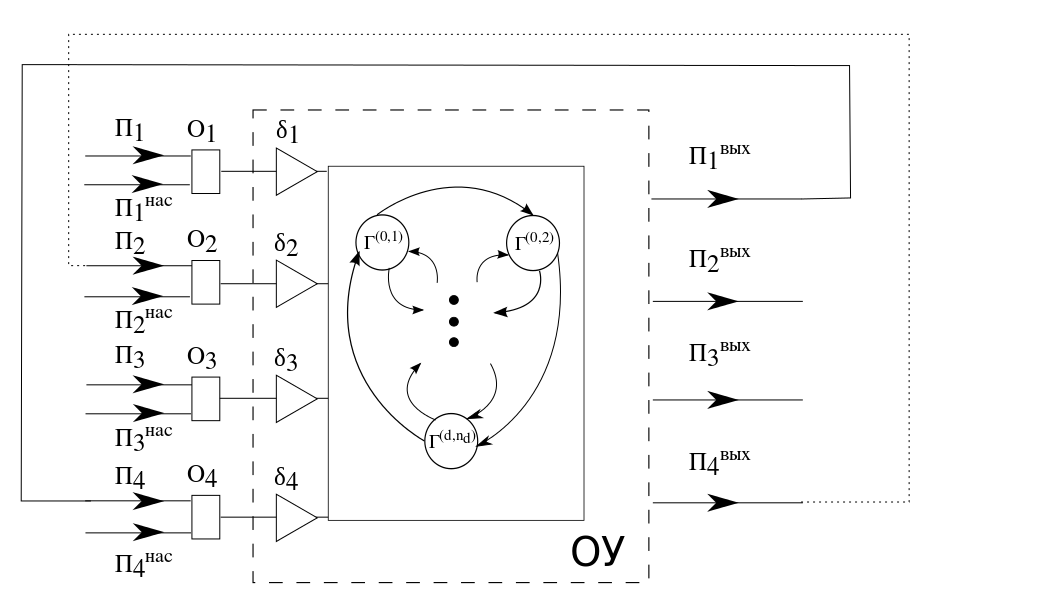
\includegraphics[scale=0.45]{SystemScheme.png} 
\caption{Структурная схема системы обслуживания}
\label{SystemScheme}
\end{figure}
В систему с одним обслуживающим устройством поступают потоки $\Pi_1$, $\Pi_2$, $\Pi_3$  и $\Pi_4$. Требования по потоку $\Pi_j$ становятся в соответствующую очередь $O_j$ с неограниченной вместимостью, $j\in \{1, 2, 3, 4\}$. Для $j \in \{1, 2, 3, 4\}$ дисциплина очереди $O_j$, поддерживаемая устройством $\delta_j$, имеет тип FIFO (First In First Out). Таким образом, для обслуживания из соответствующей очереди выбирается то требование, которое пришло раньше. Входные потоки $\Pi_1$ и $\Pi_3$ формируются внешней средой, которая, будем предполагать, имеет только одно состояние, то есть вероятностная структура потоков не меняется с течением времени. Требования потоков $\Pi_1$ и $\Pi_3$ формируют независимые между собой неординарные пуассоновские потоки, то есть  стационарные, без последействия и ординарные потоки групп требований. Обслуженные требования потока $\Pi_1$ поступают на повторное обслуживание, формируя на выходе поток $\Pi_4$. Обслуженные требования потока $\Pi_4$ в свою очередь поступают на повторное обслуживание, формируя при этом поток $\Pi_2$.  Основными параметрами системы являются: интенсивности $\lambda_1>0$, $\lambda_3>0$ поступления групп требований по потокам  $\Pi_1$, $\Pi_3$ соответственно; производящая функция распределения $f_j(z) = \sum_{\nu=1}^{\infty} p_{\nu}^{(j)} z ^{\nu}$, $|z|<(1+\varepsilon)$, $\varepsilon>0,$ числа заявок в группе по потоку $\Pi_j$, $j \in \{1,3\}$; время $T^{(k,r)}>0$  нахождения обслуживающего устройства в состоянии $\Gamma^{(k,r)}$, $k\in \{0, 1, \ldots, d\}$, $r \in \{1, 2, \ldots, n_k\}$; $\ell(k,r,j)\geqslant 0$~--- количество требований содержащихся в потоке насыщения $\Pi^{\text{нас}}_j$ в состоянии  $\Gamma^{(k,r)}$; 
 порог $L > 0$ числа требований в очереди $O_3$, при превышении которого начинается обслуживание очереди $O_3$.
 
 В каждый момент времени обслуживающее устройство находится в одном из конечного множества состояний $\Gamma=\{\Gamma^{(k,r)} \colon k=\overline{0,d}; r=\overline{1,n_k}\}$ с заданными натуральными числами $d$, $n_0$, $n_1$, $\ldots$, $n_d$. Множество состояний обслуживающего устройства разделено на $d+1$ подмножества, каждое из которых является циклом. Цикл с номером $0$ состоит из состояний продления, в котором требования потока $\Pi_3$ не обслуживаются. Из каждого состояния продления прибор может перейти в один из $d$ обычных циклов. Цикл с номером $i$ имеет $n_i$ состояний, $i=\overline{0,d}$. В каждом состоянии $\Gamma^{(k,r)}$ обслуживающее устройство находится в течение времени $T^{(k,r)}$. Граф переходов задается функцией $h(\cdot, \cdot)$: $\Gamma_{i+1} = h(\Gamma_i, \varkappa_{3,i})$, $i\geqslant 0$.

В разделе 1.2 на основе качественно описанной системы строится строгая математическая модель в виде конструктивно заданного вероятностного пространства и определенного на нем случайных величин и элементов.

При построении математической модели существенно используется кибернетический подход Ляпунова-Яблонского. Его основными принципами являются: \textbf{принцип дискретности} актов функционирования управляющей системы обслуживания во времени; \textbf{принцип совместного рассмотрения} поблочного строения управляющей системы обслуживания и ее функционирования во времени; \textbf{принцип нелокальности} при описании поблочного строения управляющей системы обслуживания. Основными блоками системы являются: 1) входные полюса~--- входные потоки $\Pi_1$, $\Pi_2$, $\Pi_3$, $\Pi_4$; 2) выходные полюса~--- $\Pi^{\text{вых}}_1$, $\Pi^{\text{вых}}_2$, $\Pi^{\text{вых}}_3$, $\Pi^{\text{вых}}_4$; 3) внешняя память~--- очереди $O_1$, $O_2$, $O_3$, $O_4$; 4) внутренняя память~--- обслуживающее устройство; 5) устройство по переработке внешней памяти~--- устройство, поддерживающее дисциплину очереди $\delta_1$, $\delta_2$, $\delta_3$, $\delta_4$; 6) устройство по переработке внутренней памяти~--- граф переходов между состояниями обслуживающего устройства; 7) внешняя среда, имеющая только одно состояние.

Для задания информации блоков вводятся следующие величины и элементы, а также указываются множества их возможных значений. В качестве дискретной временной шкалы выбрана последовательность $\tau_0=0$, $\tau_1$, $\tau_2$, $\ldots$ моментов смены состояния обслуживающего устройства. Обозначим $\Gamma_i$, $i\geqslant 1$, из множества $\Gamma$ состояние обслуживающего устройства в течение времени $\left(\tau_{i-1};\tau_i\right]$ и $\Gamma_0\in \Gamma$~--- в момент времени $\tau_0$, количество $\varkappa_{j,i} \in \mathbb{Z}_+ $, $i\geqslant 0$, требований в очереди $O_j$ в момент времени $\tau_i$, количество $\eta_{j,i} \in \mathbb{Z}_+$, $i\geqslant 0$, требований, поступивших в очередь $O_j$ по потоку $\Pi_j$ в течение времени $\left(\tau_{i};\tau_{i+1}\right]$, количество $\xi_{j,i} \in \mathbb{Z}_+$, $i\geqslant 0$, требований по потоку насыщения $\Pi^{\mathrm{\text{нас}}}_j$ в течение времени $\left(\tau_{i};\tau_{i+1}\right]$, количество $\overline{\xi}_{j,i}\in \mathbb{Z}_+$, $i\geqslant 0$, реально обслуженных требований по потоку $\Pi_j$ в течение времени $\left(\tau_{i};\tau_{i+1}\right]$; $j=\overline{1,4}$.

В завершении постановки задачи формулируются функциональные и вероятностные соотношения, которым подчиняются введеные случайные величины. А именно, из физических предположений, верны равенства:
\begin{equation}
\begin{aligned}
\overline{\xi}_{j,i}&=\min\{\varkappa_{j,i}+\eta_{j,i},\xi_{j,i}\}, \quad & \varkappa_{j,i+1}&=\varkappa_{j,i}+\eta_{j,i}-\overline{\xi}_{j,i},  \\
\varkappa_{j,i+1}&=\max\{{0,\varkappa_{j,i}+\eta_{j,i}-\xi_{j,i}}\}, \quad & \varkappa_{4,i+1}&=\varkappa_{4,i}+\eta_{4,i}-\eta_{2,i}, \\
\xi_{4,i} & = \varkappa_{4,i}, & \eta_{4,i} & = \min\{ \varkappa_{1,i} + \eta_{1,i}, \xi_{1,i}\}.
\end{aligned}
\label{rekk}
\end{equation}


При помощи разложений $\sum_{\nu=0}^{\infty} z^\nu\varphi_j(\nu,t) = \exp\{\lambda_j t (f_j(z)-1)\}$ и $\psi(k;y,u)=C_y^k u^k (1-u)^{y-k}$ вводятся функции $\varphi_j(\cdot,\cdot)$, $j\in \{1,3\}$, и $\psi(\cdot, \cdot, \cdot)$. Пусть $a=(a_1, a_2, a_3, a_4) \in \mathbb{Z}_+^4$ и $x=(x_1, x_2, x_3, x_4) \in \mathbb{Z}_+^4$.
Тогда вероятность $\varphi(a,k,r,x)$ одновременного выполнения равенств $\eta_{1,i}=a_1$, $\eta_{2,i}=a_2$, $\eta_{3,i}=a_3$, $\eta_{4,i}=a_4$ при условии  $\nu_i=(\Gamma{(k,r)}; x)$ есть 
\begin{equation}
\!\!\varphi_1(a_1,h_T(\Gamma^{({k},{r})},x_3)) \times \psi(a_2,x_4, p_{\tilde{k},\tilde{r}}) \times \varphi_3(a_3,h_T(\Gamma^{({k},{r})},x_3))
\times \delta_{a_4,\min{\{\ell(\tilde{k},\tilde{r},1), x_1+a_1}\}},
\label{rekk:1}
\end{equation}
%\end{block}
где $\Gamma^{(\tilde{k},\tilde{r})}=h(\Gamma^{(k,r)},x_3)$ и $\delta_{i,j}$ есть индикатор события $i=j$.

Пусть $b=(b_1, b_2, b_3, b_4) \in \mathbb{Z}_+^4$. 
Тогда вероятность $\zeta(b, k, r, x)$ одновременного выполнения равенств $\xi_{1,i}=b_1$, $\xi_{2,i}=b_2$, $\xi_{3,i}=b_3$, $\xi_{4,i}=b_4$ при фиксированном значении метки $\nu_i=(\Gamma{(k,r)}; x)$ есть
\begin{equation}
\delta_{b_1,\ell(\tilde{k},\tilde{r},1)} \times \delta_{b_2,\ell(\tilde{k},\tilde{r},2)} \times 
\delta_{b_3,\ell(\tilde{k},\tilde{r},3)} \times \delta_{b_4,x_4}.
\label{rekk:2}
\end{equation}
где $\tilde{k}$ и $\tilde{r}$ такие, что $\Gamma^{(\tilde{k},\tilde{r})}=h(\Gamma^{(k,r)},x_3)$.

Основным результатом первой главы является теорема 1.1, доказательство которой основывается на доказательстве теоремы Ионеску Тулча.

    {\bf Теорема 1.1} { 
    Пусть 
    $$\gamma_0=\Gamma^{(k_0,r_0)} \in \Gamma, \quad x^0=(x_{1,0},x_{2,0}, x_{3,0},x_{4,0})\in \mathbb{Z}_+^4$$ фиксированы. Тогда существует вероятностное пространство $(\Omega, {\cal F}, {\mathbf P}(\cdot))$ и заданные на нем случайные величины $\eta_{j,i}=\eta_{j,i}(\omega)$, $\xi_{j,i}=\xi_{j,i}(\omega)$, $\overline{\xi}_{j,i}=\xi_{j,i}(\omega)$, $\varkappa_{j,i}=\varkappa_{j,i}(\omega)$ и случайные элементы $\Gamma_i=\Gamma_i(\omega)$, $i\geqslant 0$, $j\in \{1, 2, 3, 4\}$, такие, что 
    \begin{itemize}
    \item имеют место равенства $\Gamma_0(\omega) = \gamma_0$ и $\varkappa_0(\omega)=x^0$;
    \item выполняются соотношения \eqref{rekk}, \eqref{rekk:1}, \eqref{rekk:2};
    \item для любых  $a$, $b$, $x^t=(x_{1,t},x_{2,t},x_{3,t},x_{4,t}) \in \mathbb{Z}_+^4$, $\Gamma^{(k_t,r_t)} \in \Gamma$, $t = 1, 2, \ldots$, условное распределение векторов $\eta_i$, и $\xi_i$ имеет вид 
\begin{multline*}
    {\mathbf P}(\{ \omega \colon \eta_i = a, \xi_i=b\} |\cap_{t=0}^{i}\{\omega\colon \Gamma_t=\Gamma{(k_t,r_t)}, \varkappa_t=x^t\})=\\
=\varphi(a,k_i,r_i,x^i)\times \zeta(b,k_i,r_i,x^i).
\end{multline*}
    \end{itemize}
}

\underline{\textbf{Вторая глава}} касается  анализа последовательности 
\begin{equation}
\{(\Gamma_i, \varkappa_{1,i}, \varkappa_{2,i}, \varkappa_{3,i}, \varkappa_{4,i}); i \geqslant 0\}
\label{all:sequence}
\end{equation}
Основываясь на результатах главы~1, в разделе 2.1 доказывается марковость основной последовательности и находятся выражения для ее переходных вероятностей. Вид соотношений для переходных вероятностей приводится в теореме 2.3.

 {\bf Теорема 2.3}
{ 
Пусть $x$, $\tilde{x}\in \mathbb{Z}_+^4$ и $\Gamma^{(k,r)}$, $\Gamma^{(\tilde{k},\tilde{r})}=h(\Gamma^{(k,r)},x_3) \in \Gamma$. Тогда переходные вероятности однородной счетной марковской цепи $\Mark$ вычисляются по следующей формуле:
\begin{multline*}
\Pr (\{\omega\colon \Gamma_{i+1}=\Gamma^{(\tilde{k},\tilde{r})},\varkappa_{i+1}=\tilde{x} \}| \{\omega\colon \Gamma_{i}=\Gamma^{(k,r)},\varkappa_i=x\})=\\ 
=\widetilde{\varphi}_3(\tilde{k},\tilde{r},h_T(\Gamma^{(k,r)},x_3),x_3,\tilde{x}_3)\times \\ \times
\sum_{(a_1,a_2)\in {\mathbb A}_{\mathrm{trans}}}\varphi_1(a_1,h_T(\Gamma^{(k,r)},x_3))  \psi(a_2,x_4, p_{\tilde{k},\tilde{r}}).
\end{multline*}
}

Существенно использование при выводе рекуррентных соотношений множеств особого вида:
\begin{align*}
{\mathbb A}_{\mathrm{trans}}(x,\tilde{x},\tilde{k},\tilde{r}) &= {\mathbb A}_{\mathrm{trans}}^0(x,\tilde{x},\tilde{k},\tilde{r}) \cap {\mathbb A}_{\mathrm{trans}}^1(x,\tilde{x},\tilde{k},\tilde{r})\cap {\mathbb A}_{\mathrm{trans}}^2(x,\tilde{x},\tilde{k},\tilde{r}),\label{A:trans:1}\\
{\mathbb A}_{\mathrm{trans}}^0(x,\tilde{x},\tilde{k},\tilde{r}) &= \{(a_1,a_2) \in \mathbb{Z}_+^2 \colon a_2 = \min{\{\ell(\tilde{k},\tilde{r},1), x_1+a_1}\} +x_4-\tilde{x}_4\},\\
{\mathbb A}_{\mathrm{trans}}^1(x,\tilde{x},\tilde{k},\tilde{r}) &= \{(a_1,a_2) \in \mathbb{Z}_+^2 \colon \tilde{x}_1=\max{\{0,x_1+a_1-\ell(\tilde{k},\tilde{r},1)\}}\},\\
{\mathbb A}_{\mathrm{trans}}^2(x,\tilde{x},\tilde{k},\tilde{r}) &= \{(a_1,a_2) \in \mathbb{Z}_+^2 \colon  \tilde{x}_2=\max{\{0,x_2+a_2-\ell(\tilde{k},\tilde{r},2)\}}\}.
\end{align*}

В разделе 2.2 проводится классификация состояний марковской цепи \eqref{all:sequence} по арифметических свойствам. 

    Для классификации состояний необходимо определить взаимную достижимость состояний цепи  $\Mark$.
    Например, сообщаются ли состояния
    вида $$(\Gamma^{(0,r_0)},x^0), \quad r_0=\overline{1,n_0}, \quad x^0 \in \mathbb{Z}_+^4,\quad x_{3,0} \leqslant L$$
   с состояниями вида   $$(\Gamma^{(0,\tilde{r})},(0,0,\tilde{x}_3,0)), \quad \tilde{r} = \overline{1,n_0}, \quad \tilde{x}_3\geqslant x_{3,0}.$$
    
Лемма 2.1 дает ответ на этот вопрос.

 {\bf Лемма 2.1}
{
Для любых состояний $(\Gamma^{(0,r_0)},x^0)$, $r_0=\overline{1,n_0}$, $x^0 \in \mathbb{Z}_+^4$, $x_{3,0} \leqslant L$, и $(\Gamma^{(0,\tilde{r})},(0,0,\tilde{x}_3,0))$, $\tilde{r} = \overline{1,n_0}$, $\tilde{x}_3\geqslant x_{3,0}$, существует такое натуральное число $N$, что 
\begin{equation*}
\Pr(\{\omega\colon\Gamma_{N}=\Gamma^{(0,\tilde{r} )}, \varkappa_{N}=(0,0,\tilde{x}_3,0)\}|
\{\omega\colon\Gamma_{0}=\Gamma^{(0,r_0)}, \varkappa_{0}=x^0\})>0.
\end{equation*}
}

Далее, последовательно рассматривая все состояния, Леммы 2.1~-- 2.9 подводят к основному результату главы 2.
    
 {\bf Теорема 2.5}
{\it 
Состояния вида
$(\Gamma^{(\tilde{k},\tilde{r})},\tilde{x})$,
где $\tilde{k}=\overline{0,d}$, $\tilde{r} = \overline{1,n_{\tilde{k}}}$, $\tilde{x}\in \mathbb{Z}_+^4$,
\begin{gather*}
(\tilde{x}_1>0) \Rightarrow (\tilde{x}_4\geqslant \ell(\tilde{k},\tilde{r},1)),\label{reachable:1}\\
\tilde{x}_3\geqslant \max{\Bigl\{0,L+1-\sum_{s=1}^{\tilde{r}}\ell(k,s,3)\Bigr\}}, \text{ если } \tilde{k}>0,\\
\tilde{x}_3\geqslant \max{\Big\{0,L+1-\max_{k=\overline{1,d}}{\{\sum_{s=1}^{n_{\tilde{k}}} \ell(\tilde{k},s,3)\}}\Bigr\}}, \text{ если } \tilde{k}=0,
\end{gather*}
 и только они достижимы из состояния $(\Gamma^{(0,r_0)},x^0)$, $x^0=(0,0,L+1,0)$, $r_0=\overline{1,n_0}$, и, следовательно, являются существенными.
 \label{important:states:basic}
}

В этой теореме решается вопрос о множестве существенных состояний марковской цепи $\Mark$

Очереди $O_1$ и $O_3$ первичных требований и промежуточная очередь $O_4$ исследованы в \underline{\textbf{третьей главе}}. В связи со сложностью общей модели, включающей все очереди $O_1$, $O_2$, $O_3$, $O_4$, для поиска условий стационарности необходимо разбить эту задачу на несколько подзадач.

В разделе 3.1 достаточное условие ограниченности последовательности математических ожиданий $\{E\varkappa_{4,i}(\omega); i =0, 1, \ldots\}$  представлено в теореме~3.1.

 {\bf Теорема 3.1}
{\it 
Для того, чтобы последовательность $\{E\varkappa_{4,i}(\omega); i =0, 1, \ldots\}$ была ограничена, достаточно выполнения неравенства
\begin{equation*}
   % \min_{\substack{k=\overline{1,d}\\ j=1,3}} {\{p_{k,r}\}} > 0.
    \min_{k=\overline{0,d}, r=\overline{1,n_k}} {\{p_{k,r}\}} > 0.
\end{equation*}
}

В разделе 3.2 начинается анализ последовательности $\MarkThree$. Более точно, находятся рекуррентные соотношения для производящих функций $
\mathfrak{M}^{(3,i)}(k,r,v) = \sum_{w=0}^{\infty} Q_{3,i}(\Gamma^{(k,r)},w) v^w
$, $\Gamma^{(k,r)}\in \Gamma$. 
Найденные соотношения в свою очередь используются при нахождении условий существования стационарного распределения последовательности $\MarkThree$. Теорема 3.4 раздела 3.3 содержит достаточное условие стационарности.

 {\bf Теорема 3.4}
{ 
Для того, чтобы марковская цепь $\MarkThree$ имела стационарное распределение $Q(\gamma,x)$, $(\gamma,x)\in \Gamma \times {\mathbb Z}_+$, достаточно выполнения неравенства 
\begin{equation*}
\min_{k=\overline{1,d}} { \frac{\sum_{r = 1}^{n_k} \ell(k,r,3) }{\lambda_3 f_3'(1) \sum_{r=1}^{n_k} T^{(k,r)} }}>1.
\label{sufficient:low}
\end{equation*}
}

И далее теорема 3.5 раздела 3.4 содержит необходимое условие существования стационарного распределения.

 {\bf Теорема 3.5}
{
Для того, чтобы марковская цепь $\MarkThree$ имела стационарное распределение $Q_3(\gamma,x)$, $(\gamma,x)\in \Gamma \times {\mathbb Z}_+$, необходимо выполнение неравенства
$$
\max_{k=\overline{1,d}} { \frac{\sum_{r = 1}^{n_{k}}\ell(k,r,3)}{\lambda_3 f_3'(1) \sum_{r = 1}^{n_k} T^{(k,r)}} } >1.
$$
}

Завершает теоретические исследования работы раздел 3.5, содержащий анализ последовательности $\{(\Gamma_i, \varkappa_{1,i},\varkappa_{3,i}); i \geqslant 0\}$. В теореме 3.8 приведено описание множества сущетсвенных состояний цепи.


{\bf Теорема 3.8}
Множество существенных состояний марковской цепи $\{(\Gamma_i, \varkappa_{1,i},\varkappa_{3,i});$ $i \geqslant 0\}$ имеет вид $\raisebox{-.5ex}{$\biggl($}\bigcup\limits_{1 \leqslant r \leqslant n_0}S^1_{0,r}\raisebox{-.5ex}{$\biggr)$}\cup \raisebox{-.5ex}{$\biggl($}\bigcup\limits_{\substack{1 \leqslant k \leqslant d\\ 1 \leqslant r \leqslant n_k}} S^1_{k,r}\raisebox{-.5ex}{$\biggr)$}$.
где
\begin{align*}
  S^1_{0,r} = & 
  \biggl\{
  (\Gamma^{(0,r)},x_1, x_3) \colon \; (x_1, x_3)\in Z^2_+,\; x_3 > L - \max\limits_{k=1, 2,
    \ldots, d}
  \biggl\{ \sum_{t=1}^{n_k} \ell({k,t,3}) \biggl\}\biggl\}, 
  \quad 1 \leqslant r \leqslant n_0, \\
  S^1_{k,r} = & 
  \biggl\{
  (\Gamma^{(k,r)},x_1, x_3) \colon \; (x_1, x_3)\in Z^2_+,\; x_3 > L - \sum_{t=1}^{r} \ell({k,t,3})
  \biggr\}, 
  \quad 1 \leqslant k \leqslant d, \quad 1 \leqslant r \leqslant n_k.
\end{align*}

Теорема 3.9 содержит достаточное условие существования стационарного распределения марковской цепи  $\{(\Gamma_i, \varkappa_{1,i},\varkappa_{3,i}); i \geqslant 0\}$.

 {\bf Теорема 3.9}
{
Для того, чтобы марковская цепь $\{(\Gamma_i, \varkappa_{1,i},\varkappa_{3,i}); i \geqslant 0\}$ имела стационарное распределение $Q_1(\gamma,x_1,x_3)$, $(\gamma,x_1,x_3)\in \Gamma \times {\mathbb Z}^2_+$, достаточно выполнения неравенств
\begin{equation}
\min_{k=\overline{0,d}} { \frac{\sum_{r = 1}^{n_k} \ell(k,r,1) }{\lambda_1 f_1'(1) \sum_{r=1}^{n_k} T^{(k,r)} }}>1, \quad 
\min_{k=\overline{1,d}} { \frac{\sum_{r = 1}^{n_k} \ell(k,r,3) }{\lambda_3 f_3'(1) \sum_{r=1}^{n_k} T^{(k,r)} }}>1.
\label{sufficient:double}
\end{equation}
}

Наконец, в \underline{\textbf{четвертой главе}} разработана и изучена имитационная модель системы. 

Управляющими параметрами системы являются:
         длительности $T_2$ и $T_3$ сигналов второго светофора;
         длительность $T_{prol}$ сигнала продления второго светофора;
         порог продления $L$.
Показателем качества функционирования системы выбрано среднее взвешенное время ожидания произвольного требования $E \gamma$. Для определения квазистационарного режима запускаются несмещенная (<<0>>) и смещенная (<<+>>) системы: с пустыми и не пустыми начальными очередями соответственно. 

Для определения момента достижения системой квазистационарного режима 
    в конце каждого такта считаются значения
\begin{equation}
   \gamma_{j,\cdot}^0 = \frac{1}{\tilde{\mathcal{V}}_j^0}\sum_{\nu} \gamma_{j,\nu}^0, \quad \gamma_{j,\cdot}^+ = \frac{1}{\tilde{\mathcal{V}}_j^+}\sum_{\nu} \gamma_{j,\nu}^+ 
\end{equation}

Кроме того, для несмещенной системы  считаются входящий и выходящий потоки:
\begin{equation}
    F^{0}_{\text{in},1} = \sum_n \alpha^{0}_{\text{in},1,n}, \quad 
    F^{0}_{\text{out},4} = \sum_n \alpha^{0}_{\text{out},4,n},
\end{equation}
\begin{equation}
    F^{0}_{\text{in},3} = \sum_n \alpha^{0}_{\text{in},3,n}, \quad 
    F^{0}_{\text{out},3} = \sum_n \alpha^{0}_{\text{out},3,n}.
\end{equation}
Стационарный режим считается достигнутым, если выполнены все неравенства:
\begin{equation}
    \frac{|\gamma_{j,\cdot}^0 - \gamma_{j,\cdot}^+|}{\gamma_{j,\cdot}^0} < \delta_1, \quad
    \frac{F^{0}_{\text{in},1}}{F^{0}_{\text{out},4}} < \delta_2, \quad 
    \frac{F^{0}_{\text{in},3}}{F^{0}_{\text{out},3}} < \delta_3.
\end{equation}

Для подсчета результирующей оценки целевой функции используется формула
\begin{equation}
 \hat{E}\gamma=\frac{\sum_{j\in\{1,3\}} (\lambda_j \sum_{\nu\geqslant1}\nu p_{\nu}^{(j)})\hat{E}\gamma_{j} }{\sum_{j\in\{1,3\}} \lambda_j \sum_{\nu\geqslant1}\nu p_{\nu}^{(j)}},
\end{equation}
где $\hat{E}\gamma_{j}=\frac{1}{\tilde{\mathcal{V}}_j}\sum_{\nu}\zeta_{j,\nu}$  -- оценка математического ожидания времени пребывания в системе произвольного требования потока $\Pi_j$.

Проведение конкретных экспериментов показало, что найденная теоретически область стационарности может быть расширена при циклическом алгоритме с продлением на втором перекрестке. Весьма ожидаемо, что тем больше область стационарности увеличивается, чем больше пороговое значение $L$ числа машин очереди $O_3$. Интересно также, что кривая разных загрузок, определяемая для циклического алгоритма с продлением особым образом, уже не содержит в своей окрестности оптимального значения параметров управления. В противопоставление, конечно, с циклическим алгоритмом без продления.


В \underline{\textbf{ заключении }} приведены основные результаты, которые состоят в следующем:
    \begin{enumerate}
        \item построена строгая математическая модель тандема с циклическим алгоритмом управления и алгоритмом с продлением;
        \item найдены условия существования стационарного распределения для цепи, включающей низкоприоритетную очередь;
        \item найдены условия существования стационарного распределения для цепей, включающих промежуточную и первичные очереди;
        \item разработана имитационная модель для изучения исходной системы;
        \item на основе имитационной модели были подтверждены и расширены результаты, полученные теоретически.
    \end{enumerate}

\section*{Список публикаций по теме диссертации}
    % \setItemnumber{5}

    \begin{enumerate}

   \item Кочеганов~В.М., Зорин~А.В. Вероятностная модель тандема систем массового обслуживания с циклическим управлением с продлением // Теория вероятностей, случайные процессы, математическая статистика и приложения: материалы Междунар. науч. конф., посвящ. 80-летию проф., д-ра физ.-мат. наук Г.А. Медведева, Минск, 23–26 февр.~--- 2015.~--- С.~94--99.
\item Кочеганов~В.М., Зорин~А.В. Дискретная модель колебания длины низкоприоритетной очереди в тандеме систем массового обслуживания при циклическом алгоритме с продлением // Дискретные модели в теории управляющих систем: IX Международная конференция, Москва и Подмосковье, 20–22 мая.~--- 2015.~--- С.~126--129.


\item
Kocheganov~V.M., Zorine~A.V. Low-priority queue Fluctuations in Tandem of Queuing Systems Under Cyclic Control with Prolongations // DCCN. Ser. Communications in Computer and Information Science. 2016.~--- V.~601.~--- Pp.~268--279.

\item  Kocheganov~V.M., Zorine~A.V. Low-priority queue and server's steady-state existence in a tandem under prolongable cyclic service // Distributed Computer and Communication Networks. DCCN~2016. Ser. Communications in Computer and Information Science.~--- 2016.~--- V.~678.~--- Pp.~210--221.


\item Кочеганов~В.М., Зорин~А.В. Достаточное условие существования стационарного режима низкоприоритетной очереди в тандеме систем массового обслуживания // Вестник Волжской государственной академии водного транспорта.~--- 2017.~--- Выпуск~50.~--- С.~47--55.

\item 
Кочеганов~В.М., Зорин~А.В. Изучение процесса управления потоками первичных требований в тандеме систем обслуживания с циклическим алгоритмом с продлением // Проблемы теоретической кибернетики: XVIII международная конференция (Пенза, 19--23 июня 2017~г.) : Материалы : Под редакцией Ю.И.~Журавлева.~--- М.:~МАКС~Пресс.~--- 2017.~--- С.~135--137.

\item 
Кочеганов~В.М., Зорин~А.В. Анализ потоков первичных требований в тандеме при циклическом управлении с продлением // Информационные технологии и математическое моделирование (ИТММ--2017): Материалы XVI Международной конференции имени А.Ф. Терпугова (29 сентября -- 3 октября 2017 г.) -- Томск: Изд-во~НТЛ.~--- 2017.~--- Ч.~1.~--- С.81--87.

\item
Kocheganov~V., Zorine~A. Primary input flows in a tandem under prolongable cyclic service // Distributed Computer and Communication Networks. DCCN-2017.~--- 2017.~--- Pp.~517--525.

\item Кочеганов~В.М., Зорин~А.В. Достаточное условие существования стационарного режима очередей первичных требований в тандеме систем массового обслуживания // Вестник ТвГУ. Серия: Прикладная математика.~--- 2018.~--- №~2.~--- С.~49--74.
\item 
Kocheganov~V., Zorine~A.  Asymptotic properties of service and control operations in tandem systems with cyclic algorithms with prolongation // доклад включен в программу конференции ORM-2018 (октябрь, 2018 г.).
\end{enumerate}



\end{document}